\chapter{Introduction to Artificial Intelligence (AI) with Python}

\section{Introduction: Real-Life Hook}

Think about AI in everyday life:

\begin{itemize}
    \item Voice assistants like Alexa and Google Assistant  
    \item Chatbots answering questions on websites  
    \item Recommendation systems in YouTube or Netflix  
    \item Self-driving cars and facial recognition  
\end{itemize}

AI allows computers to \textbf{think, learn, and make decisions}, similar to how humans process information.

\section{Concept: What is AI?}

\begin{definition}{Artificial Intelligence}
Artificial Intelligence (AI) is the branch of computer science that enables machines to \textbf{perform tasks that usually require human intelligence}, such as learning, reasoning, problem-solving, and decision-making.
\end{definition}

\subsection{Types of AI}

\begin{itemize}
    \item \textbf{Narrow AI:} Performs specific tasks (e.g., chatbots, recommendation systems)  
    \item \textbf{General AI:} Can perform any intellectual task humans can do (still theoretical)  
\end{itemize}

\section{Python for AI}

Python is widely used in AI because of:

\begin{itemize}
    \item Simple syntax suitable for beginners  
    \item Libraries like \texttt{numpy}, \texttt{pandas}, \texttt{scikit-learn}, \texttt{tensorflow}  
    \item Active community and tutorials  
\end{itemize}

\section{Mini-Project: Simple AI Chatbot}

A beginner-friendly chatbot using basic rules:

\begin{verbatim}
# Simple rule-based chatbot
def chatbot():
    print("Hello! I am ChatBuddy. Ask me anything.")
    while True:
        user_input = input("You: ").lower()
        if "hello" in user_input:
            print("ChatBuddy: Hi there!")
        elif "your name" in user_input:
            print("ChatBuddy: I am ChatBuddy!")
        elif "bye" in user_input:
            print("ChatBuddy: Goodbye!")
            break
        else:
            print("ChatBuddy: I don't understand.")

chatbot()
\end{verbatim}

- Students learn \textbf{input processing, conditional statements, and simple AI interaction}  

\section{Concept: Machine Learning (ML) Basics}

Machine Learning is a subset of AI:

\begin{itemize}
    \item Computers learn patterns from data instead of being explicitly programmed  
    \item Example: Predicting grades based on study hours and attendance  
\end{itemize}

\subsection{Python Example: Predict Grade (Linear Regression)}

\begin{verbatim}
from sklearn.linear_model import LinearRegression
import numpy as np

# Study hours vs grades
X = np.array([[2], [4], [6], [8], [10]])  # hours
y = np.array([50, 60, 65, 70, 80])       # grades

model = LinearRegression()
model.fit(X, y)

# Predict grade for 7 hours
predicted = model.predict([[7]])
print(f"Predicted grade: {predicted[0]:.2f}")
\end{verbatim}

- Students learn \textbf{data input, training a model, and making predictions}  

\section{Step-by-Step Diagram: AI / ML Workflow}

\begin{center}
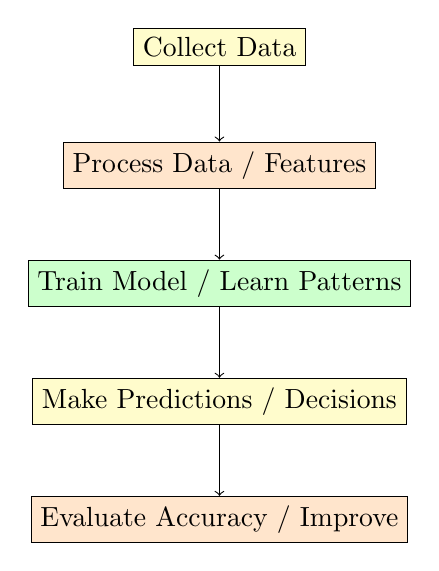
\begin{tikzpicture}[node distance=1.5cm]
\node (data) [draw, rectangle, fill=yellow!20] {Collect Data};
\node (process) [draw, rectangle, fill=orange!20, below of=data] {Process Data / Features};
\node (train) [draw, rectangle, fill=green!20, below of=process] {Train Model / Learn Patterns};
\node (predict) [draw, rectangle, fill=yellow!20, below of=train] {Make Predictions / Decisions};
\node (evaluate) [draw, rectangle, fill=orange!20, below of=predict] {Evaluate Accuracy / Improve};
\draw[->] (data) -- (process);
\draw[->] (process) -- (train);
\draw[->] (train) -- (predict);
\draw[->] (predict) -- (evaluate);
\end{tikzpicture}
\end{center}

\section{Real-Life Student Examples}

\begin{itemize}
    \item Predicting exam scores based on study hours  
    \item Recommending books based on previous reading  
    \item Simple chatbot for school website  
    \item Sorting favorite songs based on listening habits  
\end{itemize}

\section{Key Concepts}

\begin{itemize}
    \item AI enables machines to mimic human intelligence  
    \item ML is a way for computers to \textbf{learn from data}  
    \item Python libraries make AI implementation easier  
    \item Simple AI can be \textbf{rule-based or data-driven}  
\end{itemize}

\section{End-of-Chapter Exercises}

\begin{exercise}{Very Short Questions}
\begin{enumerate}
    \item What is Artificial Intelligence?  
    \item Name one Python library used for AI.  
    \item What is Machine Learning?  
\end{enumerate}
\end{exercise}

\begin{exercise}{Short Answer Questions}
\begin{enumerate}
    \item Write a simple rule-based chatbot that greets the user.  
    \item Explain the difference between AI and ML in simple terms.  
    \item Give one real-life example of AI students encounter every day.  
\end{enumerate}
\end{exercise}

\begin{exercise}{Activity-Based Questions}
\begin{enumerate}
    \item Create a Python program that predicts the marks of a student using a linear relationship between study hours and marks.  
    \item Modify the chatbot to answer 3 new questions about your school.  
    \item Collect 5 sample data points of your classmates’ favorite subjects and create a rule-based program to suggest a subject for new students.  
\end{enumerate}
\end{exercise}

\section{Teacher Notes}

\marginnote{
\textbf{Learning Objectives:}  
\begin{itemize}
    \item Students understand basic AI and ML concepts  
    \item Students can create simple rule-based AI programs  
    \item Students can experiment with small data-driven predictions  
\end{itemize}

\textbf{Teaching Tips:}  
\begin{itemize}
    \item Relate AI to familiar examples like chatbots, recommendation systems  
    \item Start with simple rule-based AI before showing data-driven ML  
    \item Encourage students to experiment and explore different inputs  
\end{itemize}

\textbf{Assessment:}  
\begin{itemize}
    \item Check functionality of chatbot or AI programs  
    \item Observe correct use of input, conditionals, and simple predictions  
\end{itemize}
}